\documentclass{sig-alternate}

\usepackage[utf8]{inputenc}
\usepackage[T1]{fontenc}
\usepackage[T1,T2A]{fontenc}
\usepackage{lmodern}
\usepackage[activate=compatibility]{microtype}

\usepackage{mathtools}
\usepackage{enumitem}
\usepackage[hyphens]{url}
\usepackage[pdftex,urlcolor=black,colorlinks=true,linkcolor=black,citecolor=black]{hyperref}
\def\sectionautorefname{Section}
\def\subsectionautorefname{Subsection}

\usepackage{graphicx}
\usepackage{caption}
\usepackage{subcaption}

\newcommand{\superscript}[1]{\ensuremath{^{\textrm{#1}}}}

% listings and Verbatim environment
\usepackage[usenames,dvipsnames,svgnames,table]{xcolor}
\usepackage{fancyvrb}
\usepackage{relsize}
\usepackage{listings}
\usepackage{verbatim}
\newcommand{\defaultlistingsize}{\fontsize{8pt}{9.5pt}}
\newcommand{\inlinelistingsize}{\fontsize{8pt}{11pt}}
\newcommand{\smalllistingsize}{\fontsize{7.5pt}{9.5pt}}
\newcommand{\listingsize}{\defaultlistingsize}
\RecustomVerbatimCommand{\Verb}{Verb}{fontsize=\inlinelistingsize}
\RecustomVerbatimEnvironment{Verbatim}{Verbatim}{fontsize=\defaultlistingsize}
\lstset{frame=lines,captionpos=b,numberbychapter=false,escapechar=§,
        aboveskip=2em,belowskip=1em,abovecaptionskip=0.5em,belowcaptionskip=0.5em,
        framexbottommargin=-1em,basicstyle=\ttfamily\listingsize\selectfont}

% use Courier from this point onward
\let\oldttdefault\ttdefault
\renewcommand{\ttdefault}{pcr}
\let\oldurl\url
\renewcommand{\url}[1]{\inlinelistingsize\oldurl{#1}}

\lstdefinelanguage{JavaScript}{
  keywords={console, log, addEventListener, onmessage, alert, push, typeof, new, true, false, catch, function, return, null, catch, switch, var, if, in, while, do, else, case, break},
  keywordstyle=\bfseries,
  ndkeywords={class, export, boolean, throw, implements, import, this},
  ndkeywordstyle=\color{darkgray}\bfseries,
  identifierstyle=\color{Maroon},
  sensitive=false,
  comment=[l]{//},
  morecomment=[s]{/*}{*/},
  commentstyle=\color{ForestGreen},
  stringstyle=\color{Blue},
  morestring=[b]',
  morestring=[b]"
}

% linewrap symbol
\usepackage{color}
\definecolor{grey}{RGB}{130,130,130}
\newcommand{\linewrap}{\raisebox{-.6ex}{\textcolor{grey}{$\hookleftarrow$}}}

% todo macro
\usepackage{color}
\newcommand{\todo}[1]{\noindent\textcolor{red}{{\bf \{TODO}: #1{\bf \}}}}

\def\plus{\texttt{+}}

\begin{document}
%
% --- Author Metadata here ---
\conferenceinfo{International Conference on Multimedia Retrieval}{2014 Glasgow, UK}
\CopyrightYear{2014} % Allows default copyright year (20XX) to be over-ridden - IF NEED BE.
%\crdata{0-12345-67-8/90/01}  % Allows default copyright data (0-89791-88-6/97/05) to be over-ridden - IF NEED BE.
% --- End of Author Metadata ---

\title{Telling Breaking News Stories from Wikipedia with Social Multimedia: A~Case Study of the 2014 Winter Olympics}

\numberofauthors{1}

\author{
% 1st. author
\alignauthor
Jon Doe\titlenote{Anonymized double blind submission in accordance with the ICMR2014 guidelines}\\%Thomas Steiner\titlenote{Thomas Steiner's second affiliation is \emph{Université de Lyon, CNRS Université Lyon~1, LIRIS, UMR5205, F-69622}}\\
  \affaddr{Random University}\\%\affaddr{Google Germany GmbH}\\\affaddr{Google Germany GmbH}\\
  \affaddr{Random Street 0, 12345 Random City}\\       %\affaddr{ABC-Str.~19, 20354 Hamburg, Germany}\\
       \email{jon.doe@example.org}%\email{tomac@google.com}
}

\maketitle
\begin{abstract}
\fontencoding{T1}\selectfont
With the ability to watch Wikipedia
and Wikidata edits in realtime,
the online encyclopedia and the knowledge base
have become increasingly used targets of research
for the detection of breaking news events.
In this paper, we present a~case study of the
\emph{2014 Winter Olympics}, where we tell the story of
breaking news events in the context of the Olympics
with the help of social multimedia
stemming from multiple social networks.
Therefore, we have extended the application
\emph{Wikipedia Live Monitor}---%
a~tool for the detection of breaking news events---%
with the capability of automatically creating
media galleries that illustrate events.
Athletes winning an Olympic competition,
a~new country leading the medal table,
or simply the Olympics themselves are all events
newsworthy enough for people to concurrently
edit Wikipedia and Wikidata---%
around the world in many languages.
The Olympics being an event of common interest,
an even bigger majority of people share the event
in a~multitude of languages on global social networks.
This sharing of moments in the form of comments and multimedia
happens either in people's role as spectators or participants
directly at one of the Olympic sites,
or as indirect second screen users
in front of their TV~sets at home.
With this work, we connect the world of
Wikipedia and Wikidata with the world of social networks,
in order to convey the spirit of the
\emph{2014 Winter Olympics},
to tell the story of victory and defeat,
and following the Olympic motto \emph{Citius, Altius, Fortius}.
\end{abstract}

\category{H.5.1}{Information Interfaces and Presentation}{Multimedia Information Systems}

%\terms{Human Factors, Languages, Measurement, Experimentation}

\keywords{Storytelling, social networks, multimedia, Wikipedia}

\section{Introduction}
\label{sec:introduction}
\fontencoding{T1}\selectfont

\subsection{Brief History of Wikipedia and Wikidata}

The free online encyclopedia \emph{Wikipedia}%
\footnote{Wikipedia: \url{http://www.wikipedia.org/}}~\cite{sanger05historywikipedia} was formally launched
on January 15, 2001 by J.~Wales
and L.~Sanger,
albeit the fundamental wiki technology
and the underlying concepts are older.
Wikipedia's direct predecessor was Nupedia%
~\cite{sanger05historywikipedia},
a~similarly free online encyclopedia,
however, that was exclusively edited by experts
following a~strict peer-review process.
Wikipedia's initial role was to serve
as a~collaborative platform for draft articles for Nupedia.
What happened in practice was that Wikipedia
rapidly overtook Nupedia as there were no peer-reviews,
and it is now a~globally successful
highly active~\cite{steiner2013bots} Web encyclopedia
available in 287 languages with overall
more than 30 million articles.%
\footnote{Wikipedia statistics: \url{http://stats.wikimedia.org/}}

\emph{Wikidata}\footnote{Wikidata: \url{http://www.wikidata.org/}}%
~\cite{vrandecic2012wikidata}
is a~free knowledge base that can be read
and edited by both humans and bots.
As Wikipedia is a~truly global effort,
sharing non-language-dependent facts
like population figures centrally
in a~knowledge base makes a~lot of sense
to facilitate international article expansion.
The knowledge base centralizes access to
and management of structured data,
such as references between Wikipedias
and statistical information that can be used in articles.
Controversial facts such as borders in conflict regions
can be added with multiple values and sources,
so that Wikipedia articles can,
dependent on their standpoint, choose preferred values.

\subsection{Social Network Sites and Multimedia}

In~\cite{boyd2007socialnetworksites},
boyd and Ellison define the term
\emph{social network site} as follows.
\textit{``We define social network sites as web-based services
that allow individuals to
\emph{(1)}~construct a~public or
semi-public profile within a~bounded system,
\emph{(2)}~articulate a~list of other users
with whom they share a~connection, and
\emph{(3)}~view and traverse their list of connections
and those made by others within the system.
The nature and nomenclature of these connections
may vary from site to site.''}
Social network sites commonly allow their users
to publish, share, and react or comment on social multimedia files
like videos or photos.
Mobile devices like smartphones or tablets
are omnipresent at all sorts of events,
enabling broad multimedia coverage.

\subsection{Hypotheses and Research Questions}

In this paper, we connect the world of
Wikipedia and Wikidata with the world of social networks
in order to convey the spirit of the
\emph{2014 Winter Olympics}.
We automatically generate different kinds of media galleries
for breaking news events around the Olympics
and evaluate the media galleries' relevance
and their visual aesthetics.
While this paper presents a~case study
of the \emph{2014 Winter Olympics},
the overall objective is to make the system domain-inde\-pendent.
We are steered by the following hypotheses.

\begin{itemize}
  \itemsep0em
  \item[(H1)] Social multimedia is suitable for illustrating
    breaking news events around the \emph{2014 Winter Olympics}.
  \item[(H2)] Given different kinds of media galleries
    for the same breaking news event
    around the \emph{2014 Winter Olympics},
    there is always one predictable preferred kind.
  \item[(H2)] The key learnings from the domain of the
    \emph{2014 Winter Olympics} can be generalized
    to other domains.    
\end{itemize}

\noindent These hypotheses lead us to the research questions below.

\begin{itemize}
  \itemsep0em
  \item[(Q1)] What breaking news event features
    determine the relevancy of the corresponding media gallery?
  \item[(Q2)] What factors determine the choice
    of the preferred media gallery kind for a~breaking news event?
\end{itemize}

The remainder of this paper is structured as follows.
\autoref{sec:enabling-tools-background} provides background
on the tools \emph{Wikipedia Live Monitor} and
\emph{Social Media Illustrator} that we have extended
in the context of this work.
\autoref{sec:media-gallery-aesthetics} introduces the topic of
and the motivation for media gallery aesthetics.
\autoref{sec:application-architecture} describes the architecture
of the present application.
\autoref{sec:evaluation-and-discussion} contains an evaluation
and a~discussion of the obtained results.
\autoref{sec:related-work} gives an overview of related work
and finally \autoref{sec:future-work-and-conclusions}
closes the paper with an outlook on future work
and conclusions.

\section{Enabling Tools Background}
\label{sec:enabling-tools-background}
\fontencoding{T1}\selectfont

With this research, we build on and extend previous research
by Steiner \emph{et~al.}, notably
the open-source applications \emph{Wikipedia Live Monitor}%
\footnote{\emph{Wikipedia Live Monitor}:
\url{http://wikipedia-irc.herokuapp.com/}}
and \emph{Social Media Illustrator}.%
\footnote{\emph{Social Media Illustrator}:
\url{http://social-media-illustrator.herokuapp.com/}}

\subsection{Wikipedia Live Monitor}

The open-source application \emph{Wikipedia Live Monitor}
was introduced by Steiner \emph{et~al.}\
in~\cite{steiner2013mjnomore}.
It monitors Wikipedia and Wikidata for concurrent edits
that it treats as signals for breaking news events.
Whenever a~human or bot changes an article
of any of the 287 Wikipedias,%
\footnote{List of Wikipedias by size:
\url{http://meta.wikimedia.org/wiki/List_of_Wikipedias}}
a~change event gets communicated by a~chat bot
over the Wikimedia IRC server (\url{irc.wikimedia.org}),%
\footnote{Raw IRC feeds of recent changes:
\url{http://meta.wikimedia.org/wiki/IRC/Channels\#Raw_feeds}}
so that parties interested in the data
can listen to the changes as they happen.
For each language version, there is
a~specific chat room following the pattern
\texttt{"\#" + language + ".wikipedia"}.
Wikipedia articles in different languages are highly interlinked.
For example, the English article
``en:2014\_Winter\_Olympics''
on the XXII Olympic Winter Games in Sochi
is interlinked with the Russian article
\fontencoding{T2A}\selectfont%
``ru:Зимние\_Олимпийские\_игры\_2014''%
\fontencoding{T1}\selectfont.
As \emph{Wikipedia Live Monitor} monitors all language versions
of Wikipedia and Wikidata in parallel,
it exploits this fact to detect \emph{concurrent edit spikes}
of Wikipedia and Wikidata article clusters covering
the same semantic concept in multiple languages.

The application thus provides us with titles of articles
that we can use as search terms for social multimedia content
on social network sites.
In the example from above, this could be
\fontencoding{T2A}\selectfont%
``Зимние Олимпийские игры 2014''%
\fontencoding{T1}\selectfont (Russian),
``2014 Winter Olympics'' (English),
``Olympische Winterspiele 2014'' (German),
or ``2014ko Neguko Olinpiar Jokoak'' (Basque), \emph{etc.}

\subsection{Social Media Illustrator}

\emph{Social Media Illustrator} is a~likewise
open-source application by Steiner \emph{et~al.},
which was introduced in%
~\cite{steiner2013meteoroid,steiner2013tocrop}.
It provides a~social multimedia search framework
that allows for searching for and extraction of
multimedia data from the social network sites
Google\texttt{+},%
\footnote{Google\texttt{+}: \url{https://plus.google.com/}}
Facebook,\footnote{Facebook: \url{https://www.facebook.com/}}
Twitter,\footnote{Twitter: \url{https://twitter.com/}}
Instagram,\footnote{Instagram: \url{http://instagram.com/}}
YouTube,\footnote{YouTube: \url{http://www.youtube.com/}}
Flickr,\footnote{Flickr: \url{http://www.flickr.com/}}
MobyPicture,\footnote{MobyPicture: \url{http://www.mobypicture.com/}}
TwitPic,\footnote{TwitPic: \url{http://twitpic.com/}}
and Wikimedia Commons.%
\footnote{Wikimedia Commons: \url{http://commons.wikimedia.org/wiki/Main_Page}}
In a~first step, it deduplicates exact- and near-duplicate
social multimedia data based on an algorithm described in%
~\cite{steiner2013clustering}.
It then ranks social multimedia data by social signals%
~\cite{steiner2013meteoroid} based on an abstraction layer
on top of the social network sites mentioned above
and, in a~final step, allows for the creation of media galleries
following aesthetic principles~\cite{steiner2012aesthetic}
of the two kinds \emph{Strict Order, Equal Size}
and \emph{Loose Order, Varying Size},
defined in~\cite{steiner2013tocrop}.

We have ported the crucial parts
of the source code of \emph{Social Media Illustrator}
from the client-side to the server-side,
enabling us now to create media galleries at scale and on demand,
based on search terms from a~patched version of \emph{Wikipedia Live Monitor}.

\section{Media Gallery Aesthetics}
\label{sec:media-gallery-aesthetics}
\fontencoding{T1}\selectfont

A~\emph{media gallery} in the context of our task of
telling breaking news stories from Wikipedia with social multimedia
is hereby defined as a~\emph{best-of} compilation of photos, videos,
and microposts%
\footnote{A~\emph{micropost} is defined as a~textual status message
on social network sites, optionally accompanied by multimedia data}
retrieved from social networks that are related to a~given event.

\subsection{Media Gallery Kinds}

For the generation of media galleries, we apply aesthetic principles
as defined by Steiner \emph{et~al.}\
in~\cite{steiner2013tocrop,steiner2012aesthetic},
particularly, we aim for the following
three visual aesthetic principles:
\emph{(i)}~a~media gallery is called \emph{balanced}
if its shape is rectangular,
\emph{(ii)}~\emph{hole-free}
if there are no gaps from missing multimedia data,
and \emph{(iii)}~\emph{order-respecting}
if multimedia data appear in insertion order.
Two kinds of media galleries were found~\cite{steiner2013tocrop}
to fulfill these principles.

\paragraph{Strict Order, Equal Size}

A~media gallery kind called \emph{Strict Order, Equal Size}
that strictly respects the insertion order
uses an algorithm that works by resizing all multimedia data
in one row to the same height and adjusting the widths
in a~way that the aspect ratios are maintained.
A~row is filled until a~maximum row height is reached,
then a~new row (with potentially different height) starts, \emph{etc.}
This media gallery kind is strictly \emph{order-respecting},
\emph{hole-free}, and can be \emph{balanced}
by adjusting the number of media items in $+1$ steps.

\paragraph{Loose Order, Varying Size}

A~media gallery kind called \emph{Loose Order, Varying Size}
uses an algorithm that works by cropping all multimedia data
to have square aspect ratios.
This allows for organizing the items in a~way such that one big square
always contains two horizontal blocks,
each with two pairs of small squares.
The media gallery is then formed by iteratively filling
big or small squares until a~square is full,
and then adding the square to the smallest column.
This media gallery kind allows any media item to become big,
while still being loosely \emph{order-respecting} and \emph{hole-free}.
Bringing the media gallery in a~\emph{balanced} state can be harder,
as depending on the shape both small and big
media items may be required.

\subsection{Why Different Media Gallery Kinds}

The main motivation for the \emph{Loose Order, Varying Size} kind
is that certain media items can be featured more prominently
by making them big, while still loosely respecting the insertion order.
Examples of to-be-featured media items can be videos,
media items with faces, media items available in High-Density quality,
or media items with interesting details~\cite{suh2003thumbnail}.
In contrast to \emph{Loose Order, Varying Size},
\emph{Strict Order, Equal Size} does not require cropping,
which allows for multimedia data outside of common aspect rations like
$1{:}1$ (square), $3{:}2$ (digital SLRs), or $3{:}4$ (iPhone)
to be properly fitted in media galleries.

\section{Application Architecture}
\label{sec:application-architecture}
\fontencoding{T1}\selectfont

The underlying application \emph{Wikipedia Live Monitor}
puts Wiki\-pedia and Wikidata article clusters
that cover the same semantic concept
in a~monitoring loop.
Article clusters stay in the monitoring loop until
their time-to-live has been reached,
\emph{i.e.}, until there are no further edits.
Some article clusters upon fulfilling the breaking news conditions
as defined in~\cite{steiner2013mjnomore}
will be reported as breaking news events.
We have patched the \emph{Wikipedia Live Monitor} source code
to have an additional social multimedia search hook in that case.
This social multimedia search hook receives as an input
the international titles of all articles
in the currently breaking article cluster as well as their URLs.
It uses them as search terms for a~patched instance
of the application \emph{Social Media Illustrator}
that runs on the same server
as the instance of \emph{Wikipedia Live Monitor}.
It is configured to always return two media galleries
for one request, one of kind \emph{Strict Order, Equal Size}
and the other of kind \emph{Loose Order, Varying Size}.
Both generated media galleries are saved to disk
for archiving purposes following a~naming scheme
that includes the media gallery kind,
the originating search terms, and the UNIX timestamp.

On the server-side, we use a~library called node-canvas%
~\cite{holowaychuk2013nodecanvas} that implements the
HTML5 canvas API~\cite{cabanier2013canvas} on the server.
This library allowed us to port the original client-side code 
used in \emph{Social Media Illustrator}
with manageable effort to the server.
The canvas API is mainly used in the deduplication algorithm%
~\cite{steiner2013clustering}
and for creating static dumps of media galleries.
Media galleries initially consist of individual images and videos
with hyperlinks to the originating microposts
as can be seen in \autoref{code:mediagalleryhtml}.
For the archived version, a~static dump
in Portable Network Graphics format
with graphical representation of the URLs
of the originating microposts is created,
an example is shown in \autoref{fig:dario-cologna}.

\begin{lstlisting}[caption={Simplified \emph{Strict Order, Equal Size}
  HTML code}, label=code:mediagalleryhtml, language=HTML]
<div id="mediaGallery" style="width: 602px;">
  <div class="mediaItem photoBorder" tabindex="1"
      style="width: 307.5px; height: 199.875px;">
    <a href="http://www.flickr.com/[...]">
      <video src="http://www.flickr.com/[...]"
          poster="http://staticflickr.com/[...]"
          class="gallery"
          style="width: 307px; height: 199px;">
      </video>
    </a>
    <img class="favicon" src="flickr.png">
  </div>
  [...]
</div>
\end{lstlisting}

This has the advantage that dumps
can be shared as photos over social network sites,
in contrast to  HTML code with typically expiring URLs
that therefore cannot be permanently shared.

\begin{figure}
  \centering
  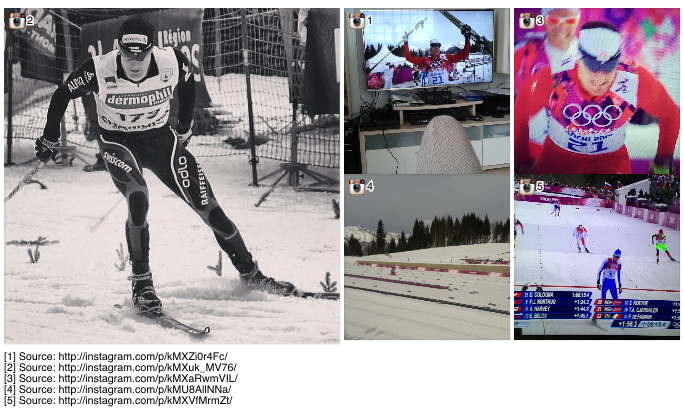
\includegraphics[width=1.0\columnwidth]{figures/dario_cologna/mediagallery_looseOrder_1391945454845.png}
  \caption{Static dump of a~media gallery of kind \emph{Loose Order, Varying Size}
  for Dario Cologna, Men's Skiathlon event gold medal winner}
  \label{fig:dario-cologna}    
\end{figure}


\section{Evaluation and Discussion}
\label{sec:evaluation-and-discussion}
\fontencoding{T1}\selectfont

\subsection{Quantitative Evaluation}

We have evaluated the application based on breaking news events
around the \emph{Winter Olympics}%
\footnote{In order to avoid confusion of the numbers,
in this section, we strip the \emph{2014} from the event title}
that happened between February~8, 20:36~(CET) and February~10, 20:38~(CET),
\emph{i.e.}, during an examination period of 48~hours.
During this period, 94~unique breaking news events
were detected by \emph{Wikipedia Live Monitor}.
Uniqueness in this context is defined as events being
reported without interruption.
For example, \emph{Christof Innerhofer} appeared twice on February~9,
once in the morning%
\footnote{Christof Innerhofer (morning):
\url{https://twitter.com/WikiLiveMon/status/432438422431887360}}
and once again in the afternoon,%
\footnote{Christof Innerhofer (afternoon):
\url{https://twitter.com/WikiLiveMon/status/432506953890537472}}
so even if the event is about the same person,
it is still tracked as two unique breaking news events.
Out of these 94~breaking news events,
69~events (${\approx}73\%$) were
related to the \emph{Winter Olympics}.
In the 48~hours of our experiment,
we have generated overall 804~media galleries,
\emph{i.e.}, 402~media galleries of kind \emph{Strict Order, Equal Size}
and accordingly 402~kind \emph{Loose Order, Varying Size}.
These 402~media gallery pairs covered 67~breaking news events---%
\emph{Winter Olympics}-related or not.
If we only count the media gallery pairs that were relevant
for the \emph{Winter Olympics},
we get 253~media gallery pairs (${\approx}63\%$)
covering 48~of the \emph{Winter Olympics} breaking news events
resulting in a~\textbf{recall of $\mathbf{{\approx}70\%}$}
(48~out of 69~of the \emph{Winter Olympics} breaking news events).
We calculate the precision in the next subsection.

\subsection{Qualitative Evaluation}

In the qualitative evaluation, we exclusively consider the 
253~media gallery pairs that illustrate the
48~\emph{Winter Olympics} breaking news events.
We have asked five independent human raters to agree on
wether a~given media gallery pair is mostly relevant or irrelevant,
or completely relevant or irrelevant for the 
\emph{Winter Olympics} breaking news event in question.
By looking at the absolute number of 253~media galleries,
78~media galleries were rated mostly irrelevant
or completely irrelevant
whereas 175~media galleries were rated mostly relevant
or completely relevant.
This results in an \textbf{absolute precision of $\mathbf{{\approx}69\%}$}.
By looking at the number of 48~\emph{Winter Olympics}-related events,
18~media gallery pairs were rated mostly irrelevant
or completely irrelevant
whereas 30~media gallery pairs were rated mostly relevant
or completely relevant, resulting in
a~\textbf{relative precision of $\mathbf{{\approx}63\%}$}.

\subsection{Aesthetic Evaluation}

In the aesthetic evaluation, we have asked the same five raters
for each of the 30~media gallery pairs
that they had previously rated mostly relevant or completely relevant
to decide on whether the \emph{Strict Order, Equal Size}
variant looked better or the \emph{Loose Order, Varying Size} variant.
Even after longer discussions between the raters,
there was no clear winner, yet each time the raters could tell exactly
what bothered them about a~given variant.
In consequence, rather than providing concrete numbers,
we decided to list the raters' most commented-on annoyances.
Media galleries of the kind \emph{Strict Order, Equal Size}
suffered badly from being unbalanced.
Rather than having more social multimedia data,
the raters would have rather preferred removing some items
in order to get to a~balanced state.
Media galleries of the kind \emph{Loose Order, Varying Size}
suffer less from being unbalanced,
but raters consistently remarked positively when they were balanced.
The biggest nuisance with \emph{Loose Order, Varying Size}
according to our raters were irregular margins
that destroy the regular grid pattern,
an example thereof can be seen in \autoref{fig:1391941759000}
in the photo of Jamie Anderson with the green-white boarder cap.
Overall, raters found \emph{Loose Order, Varying Size} media galleries
to be easier to consume, especially when the individual items were diverse.

\subsection{Temporal Evaluation}

In the temporal evaluation, we have examined the effect of 
evolution of media galleries over time.
\autoref{fig:jamie-anderson} and \autoref{fig:olga-vilukhina}
show timestamped examples of how the application
dynamically recalculates the ranking~\cite{steiner2013meteoroid}
based on the changing social signals.
As social multimedia retrieve interactions on social network sites
that we harvest whenever we generate a~new media gallery,
the algorithm takes these changes into account.
Sometimes additional multimedia data appear and
previously existing data disappear
as is the case in the step from \autoref{fig:1391960741705}
to \autoref{fig:1391960781898}.
Our raters were fascinated by the dynamics of the storytelling
where sometimes within well less than a~minute
media galleries change significantly.
They wished for ways to easily navigate back in time
in order to relive media gallery evolutions
by flipping through the versions.

\subsection{Discussion}

\todo{Discuss!}

\begin{figure}[t!]
  \centering
  % row 1
  \begin{subfigure}[t]{0.25\textwidth}
    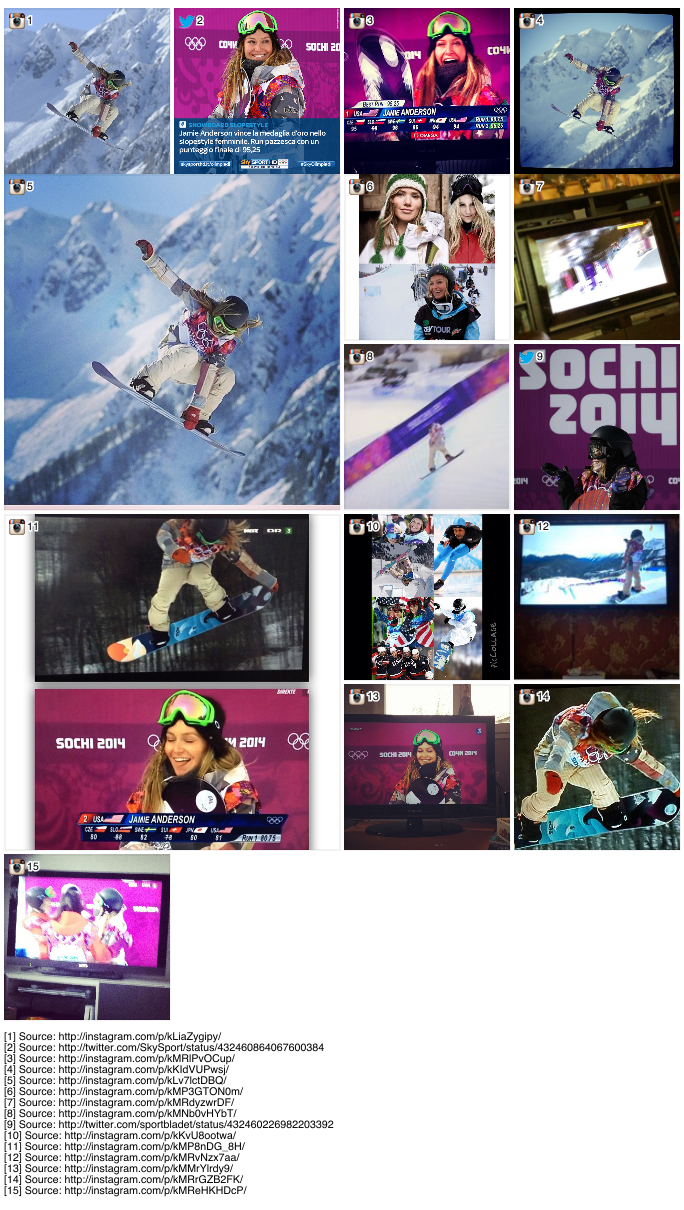
\includegraphics[height=3.75cm]{figures/jamie_anderson/mediagallery_looseOrder_1391941734592.png}
    \caption{Feb 09, 11:28:54}
    \label{fig:1391941734592}
  \end{subfigure}%
  \begin{subfigure}[t]{0.25\textwidth}
    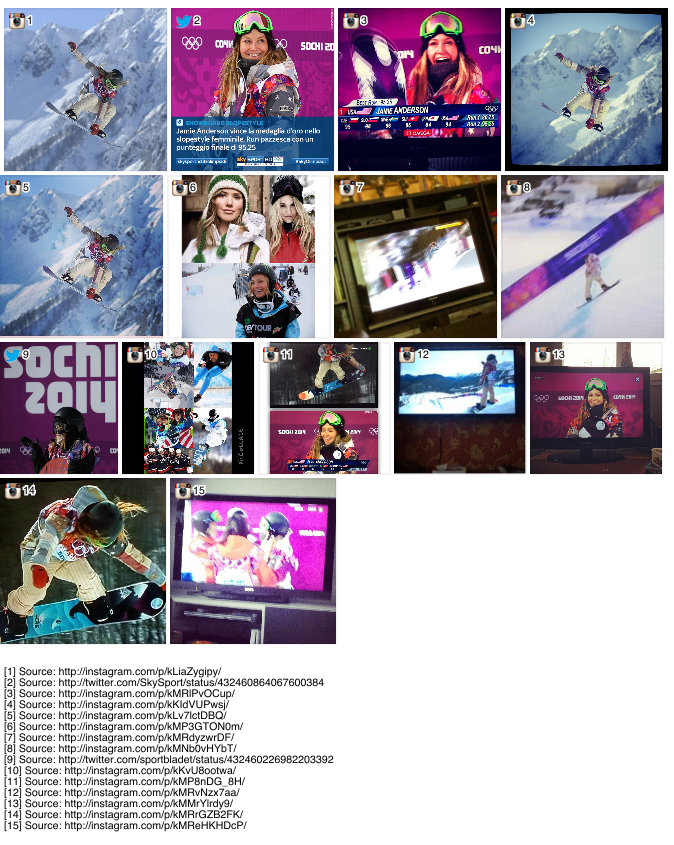
\includegraphics[height=3.75cm]{figures/jamie_anderson/mediagallery_strictOrder_1391941733935.png}
    \caption{Feb 09, 11:28:53}
    \label{fig:1391941733935}
  \end{subfigure}
  % row 2
  \begin{subfigure}[t]{0.25\textwidth}
    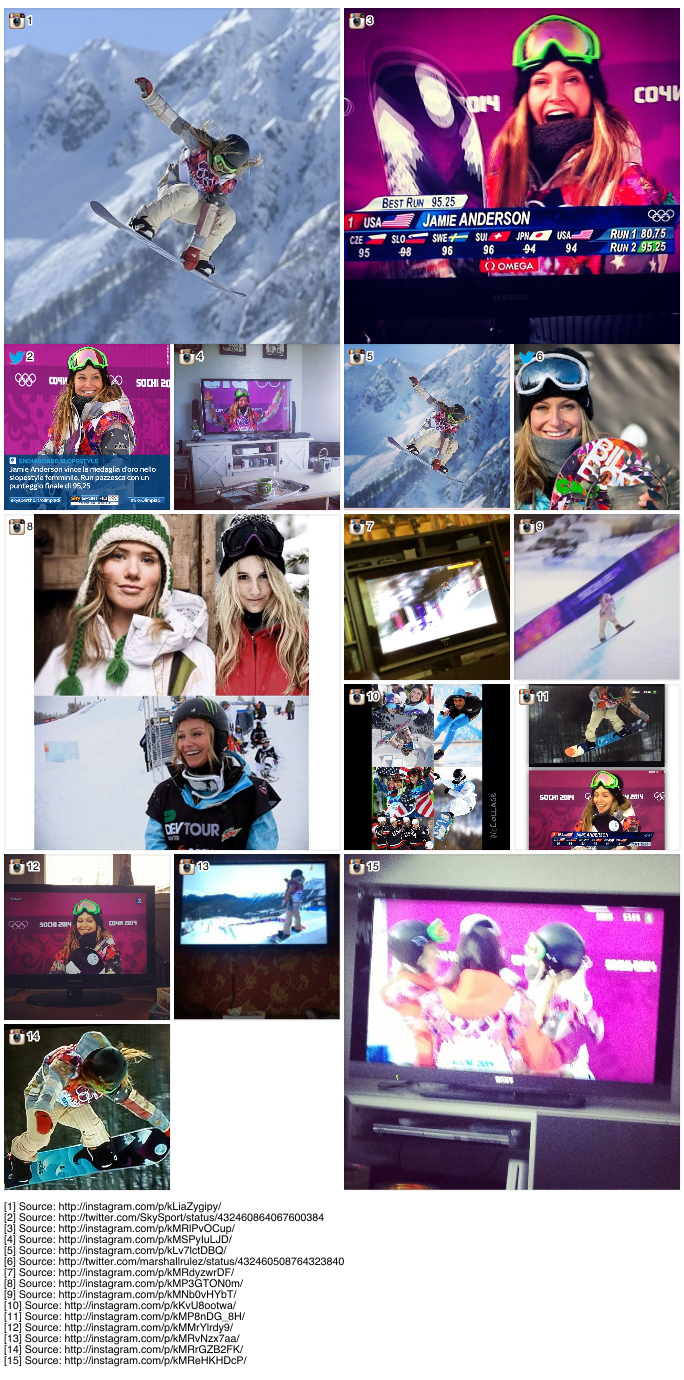
\includegraphics[height=3.75cm]{figures/jamie_anderson/mediagallery_looseOrder_1391941759000.png}
    \caption{Feb 09, 11:29:19}
    \label{fig:1391941759000}
  \end{subfigure}%
  \begin{subfigure}[t]{0.25\textwidth}
    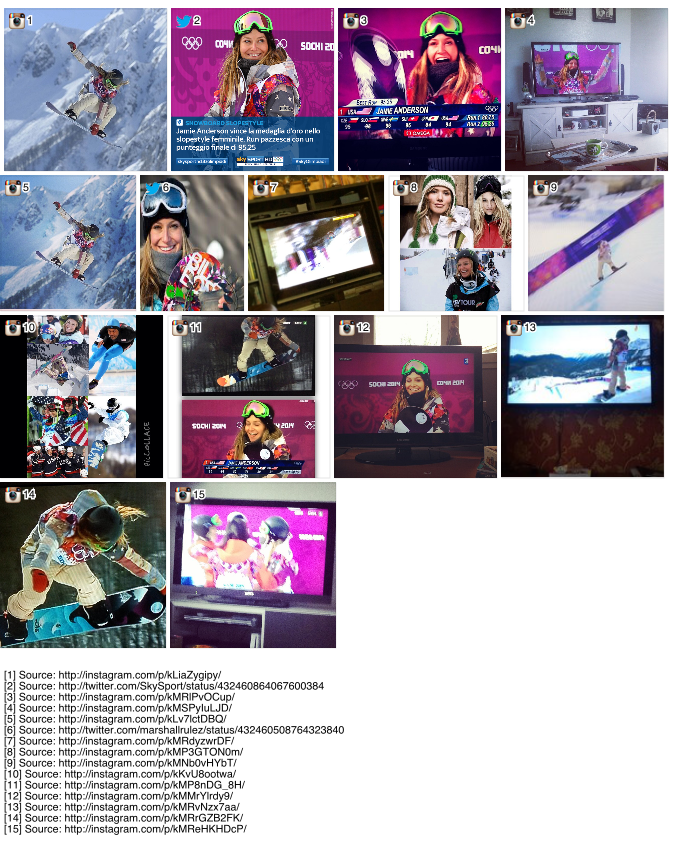
\includegraphics[height=3.75cm]{figures/jamie_anderson/mediagallery_strictOrder_1391941758324.png}
    \caption{Feb 09, 11:29:18}
    \label{fig:1391941758324}
  \end{subfigure}
  %row 3
  \begin{subfigure}[t]{0.25\textwidth}
    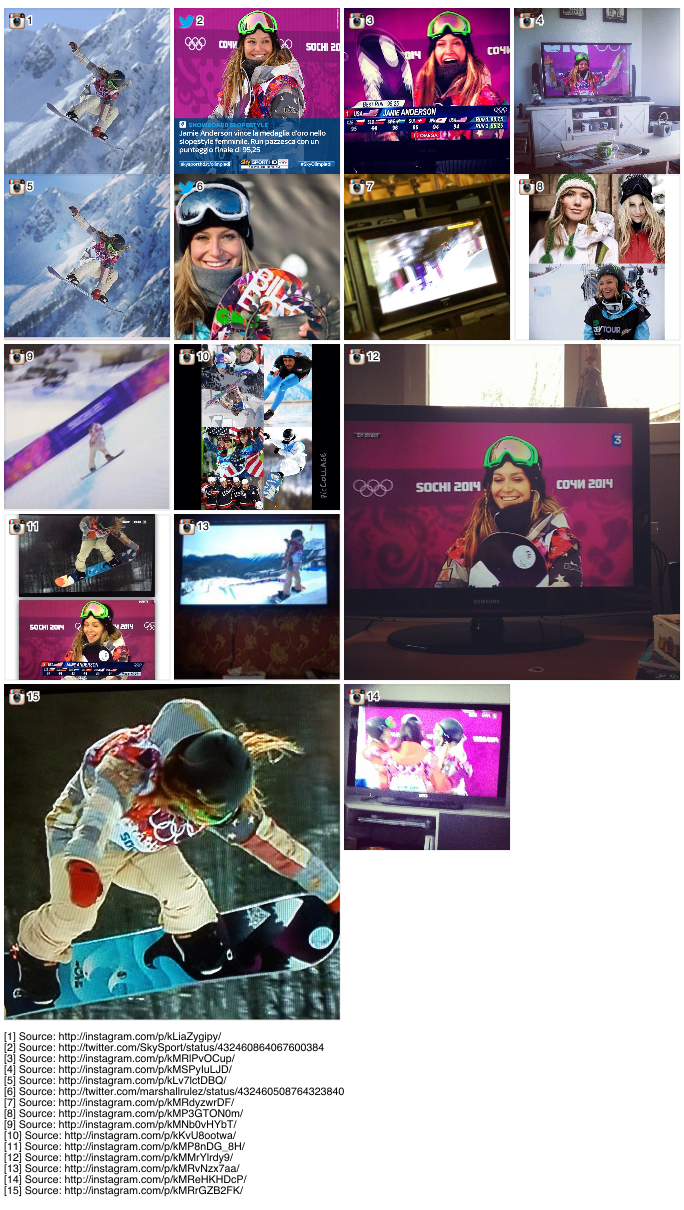
\includegraphics[height=3.75cm]{figures/jamie_anderson/mediagallery_looseOrder_1391941782689.png}
    \caption{Feb 09, 11:29:42}
    \label{fig:1391941782689}
  \end{subfigure}%
  \begin{subfigure}[t]{0.25\textwidth}
    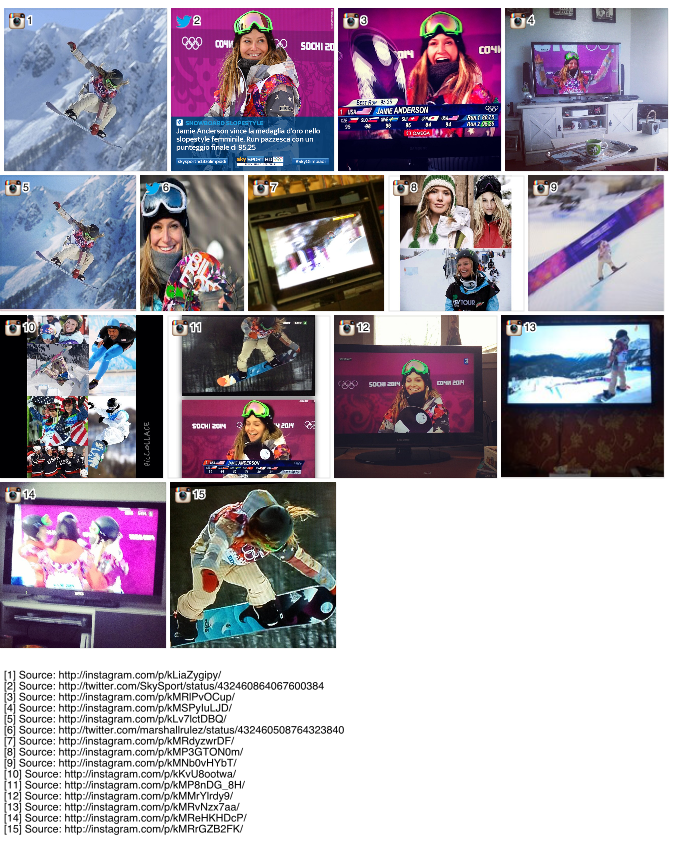
\includegraphics[height=3.75cm]{figures/jamie_anderson/mediagallery_strictOrder_1391941782536.png}
    \caption{Feb 09, 11:29:42}
    \label{fig:1391941782536}
  \end{subfigure}
  % row 4
  \begin{subfigure}[t]{0.25\textwidth}
    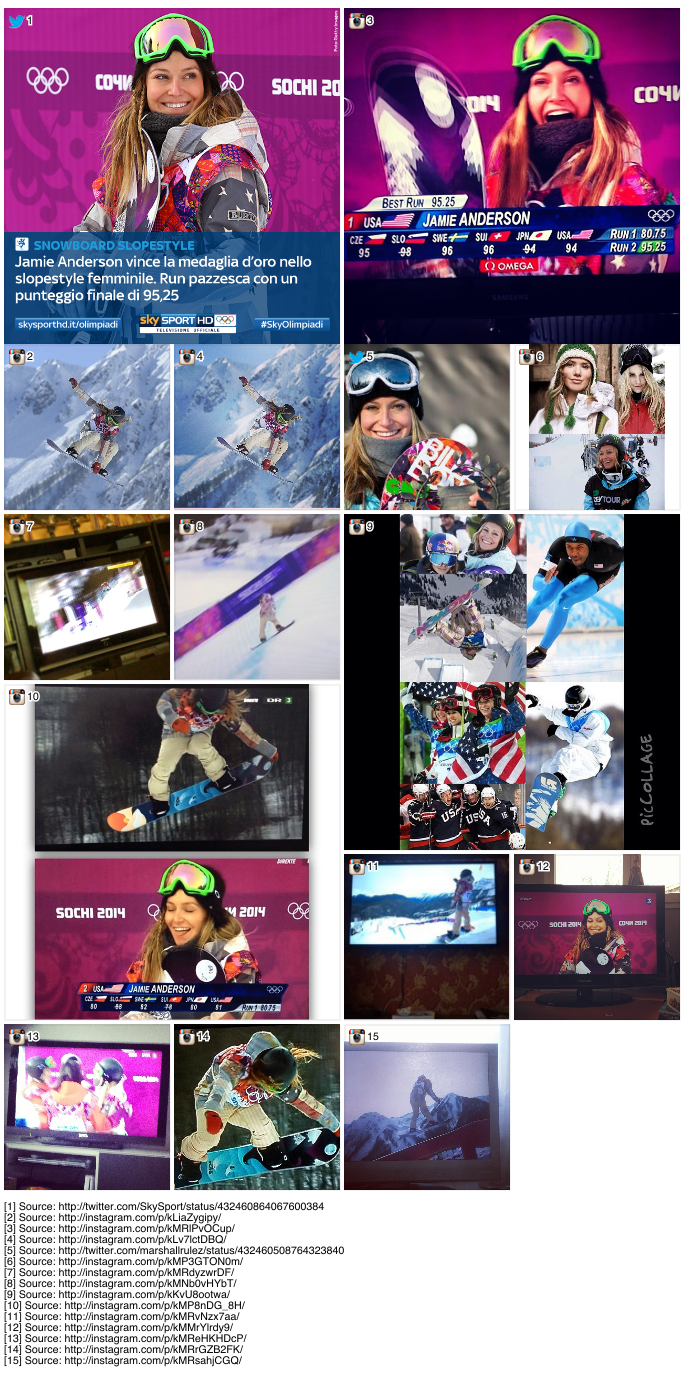
\includegraphics[height=3.75cm]{figures/jamie_anderson/mediagallery_looseOrder_1391941820404.png}
    \caption{Feb 09, 11:30:20}
    \label{fig:1391941820404}
  \end{subfigure}%
  \begin{subfigure}[t]{0.25\textwidth}
    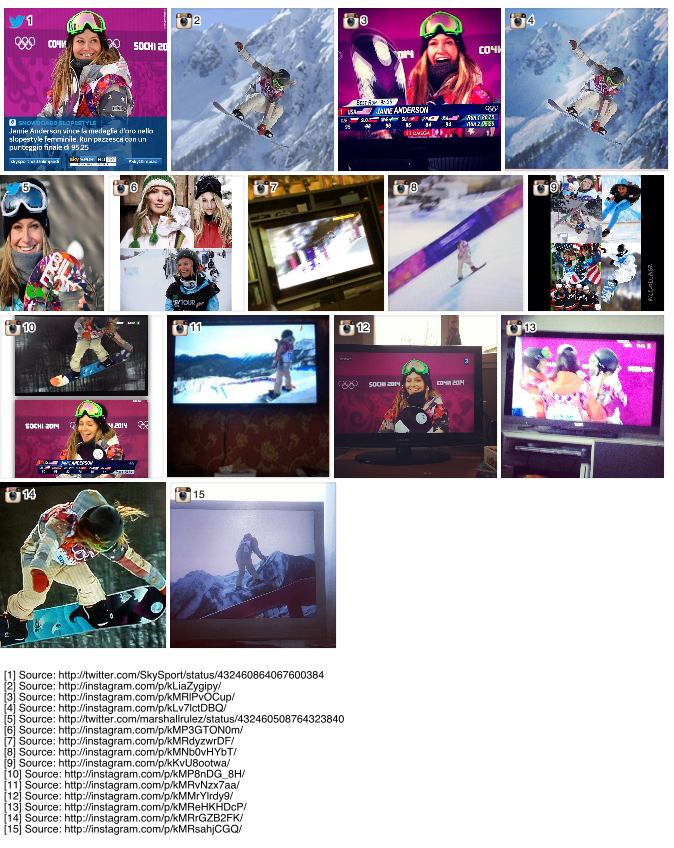
\includegraphics[height=3.75cm]{figures/jamie_anderson/mediagallery_strictOrder_1391941820162.png}
    \caption{Feb 09, 11:30:20}
    \label{fig:1391941820162}
  \end{subfigure}
  % row 5
  \begin{subfigure}[t]{0.25\textwidth}
    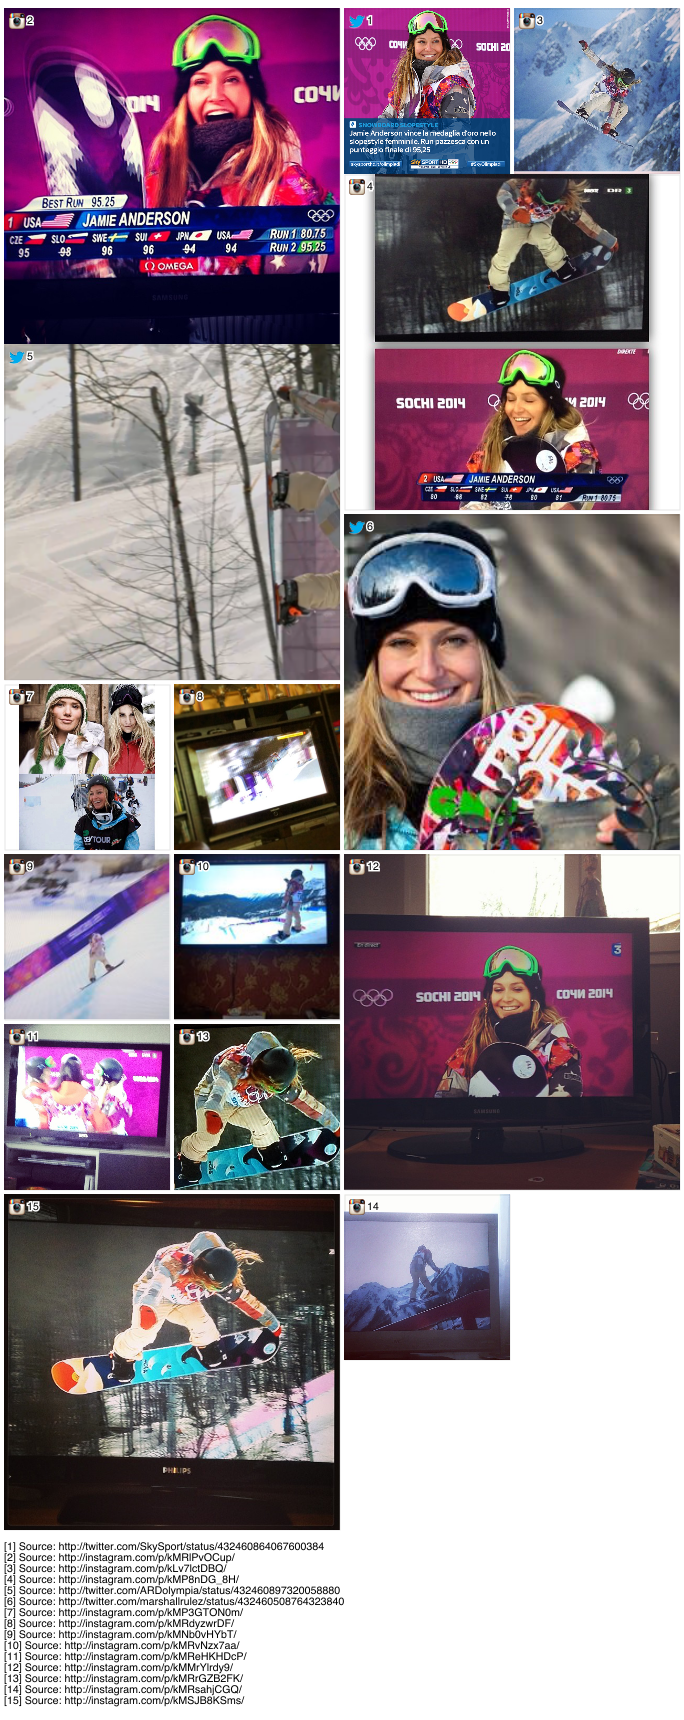
\includegraphics[height=3.75cm]{figures/jamie_anderson/mediagallery_looseOrder_1391941838760.png}
    \caption{Feb 09, 11:30:38}
    \label{fig:1391941838760}
  \end{subfigure}%
  \begin{subfigure}[t]{0.25\textwidth}
    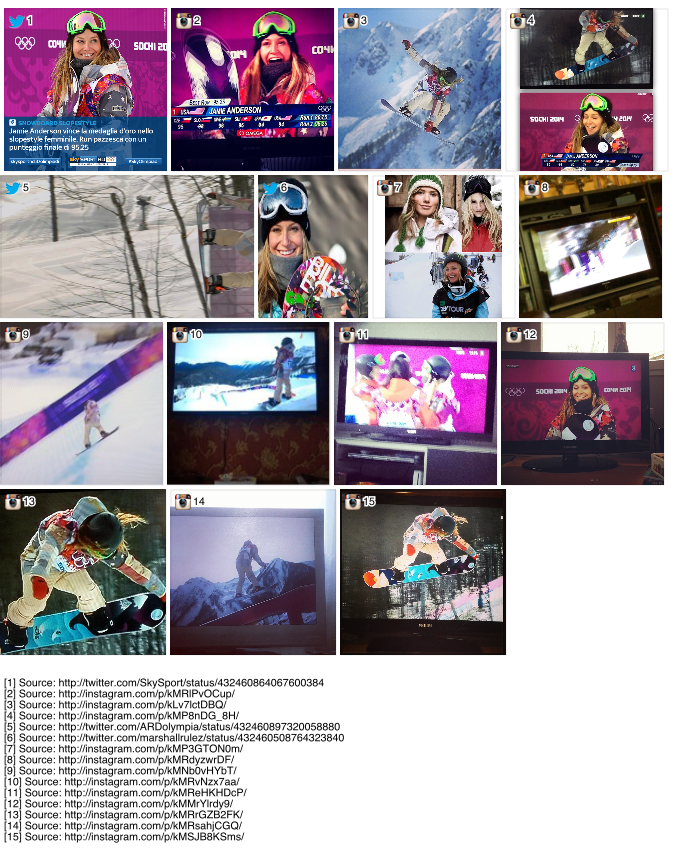
\includegraphics[height=3.75cm]{figures/jamie_anderson/mediagallery_strictOrder_1391941838444.png}
    \caption{Feb 09, 11:30:38}
    \label{fig:1391941838444}
  \end{subfigure}  
  \caption{Media galleries for Jamie Anderson,
    Women's Slopestyle Olympic gold medal winner (times in CET, left: \emph{Loose Order, Varying Size}, right: \emph{Strict Order, Equal Size})
    \url{https://twitter.com/WikiLiveMon/status/432460983676989440}}
  \label{fig:jamie-anderson}
\end{figure}

\begin{figure}[t!]
  \centering
  % row 1
  \begin{subfigure}[t]{0.25\textwidth}
    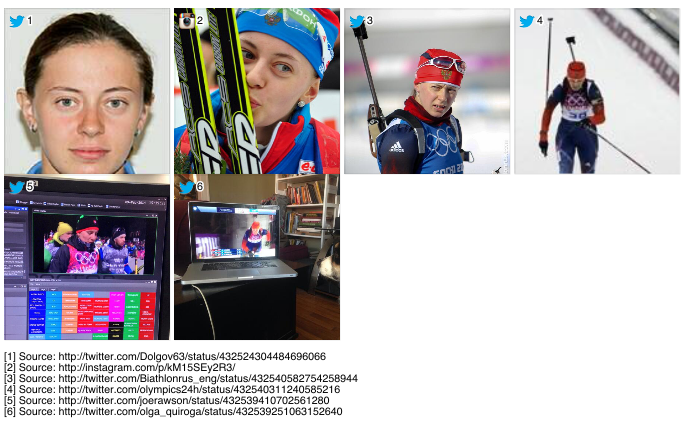
\includegraphics[height=2.75cm]{figures/olga_vilukhina/mediagallery_looseOrder_1391960736219.png}
    \caption{Feb 09, 16:45:36}
    \label{fig:1391960736219}
  \end{subfigure}%
  \begin{subfigure}[t]{0.25\textwidth}
    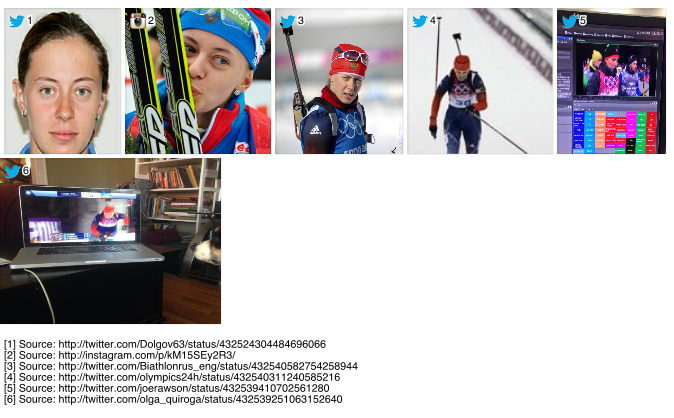
\includegraphics[height=2.75cm]{figures/olga_vilukhina/mediagallery_strictOrder_1391960736190.png}
    \caption{Feb 09, 16:45:36}
    \label{fig:1391960736190}
  \end{subfigure}
  %row 2
  \begin{subfigure}[t]{0.25\textwidth}
    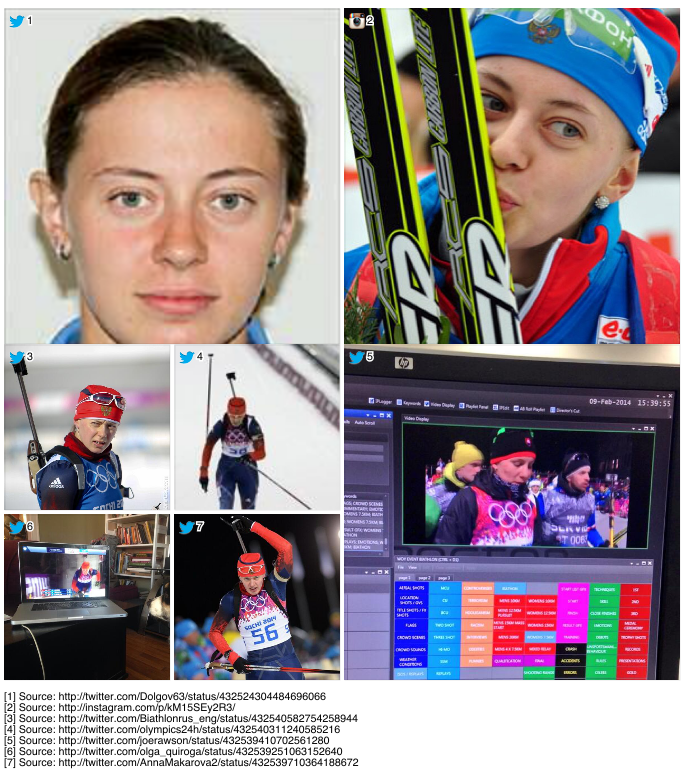
\includegraphics[height=2.75cm]{figures/olga_vilukhina/mediagallery_looseOrder_1391960742371.png}
    \caption{Feb 09, 16:45:42}
    \label{fig:1391960742371}
  \end{subfigure}%
  \begin{subfigure}[t]{0.25\textwidth}
    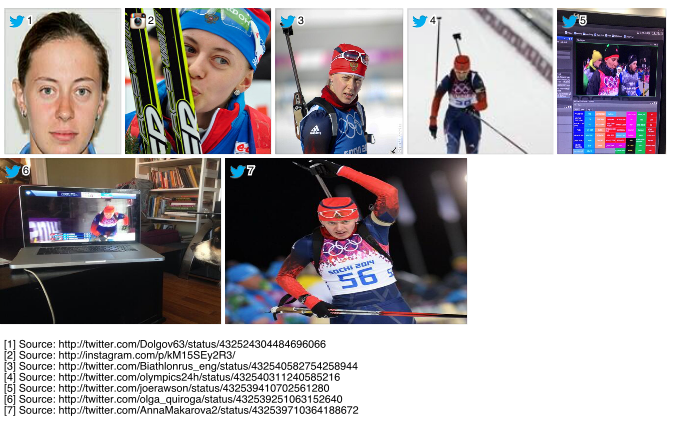
\includegraphics[height=2.75cm]{figures/olga_vilukhina/mediagallery_strictOrder_1391960741705.png}
    \caption{Feb 09, 16:45:41}
    \label{fig:1391960741705}
  \end{subfigure}
  % row 3
  \begin{subfigure}[t]{0.25\textwidth}
    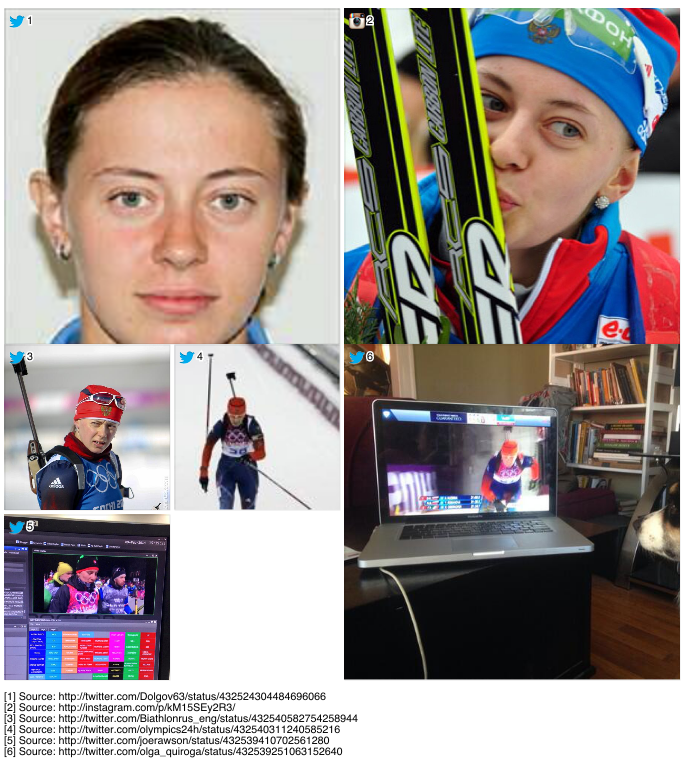
\includegraphics[height=2.75cm]{figures/olga_vilukhina/mediagallery_looseOrder_1391960782060.png}
    \caption{Feb 09, 16:46:22}
    \label{fig:1391960782060}
  \end{subfigure}%
  \begin{subfigure}[t]{0.25\textwidth}
    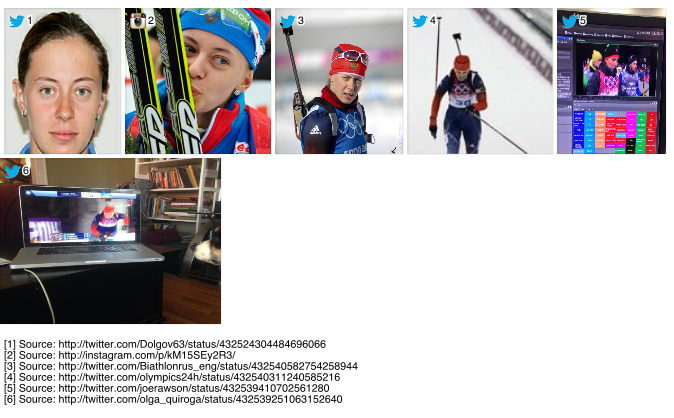
\includegraphics[height=2.75cm]{figures/olga_vilukhina/mediagallery_strictOrder_1391960781898.png}
    \caption{Feb 09, 16:46:21}
    \label{fig:1391960781898}
  \end{subfigure}
  % row 4
  \begin{subfigure}[t]{0.25\textwidth}
    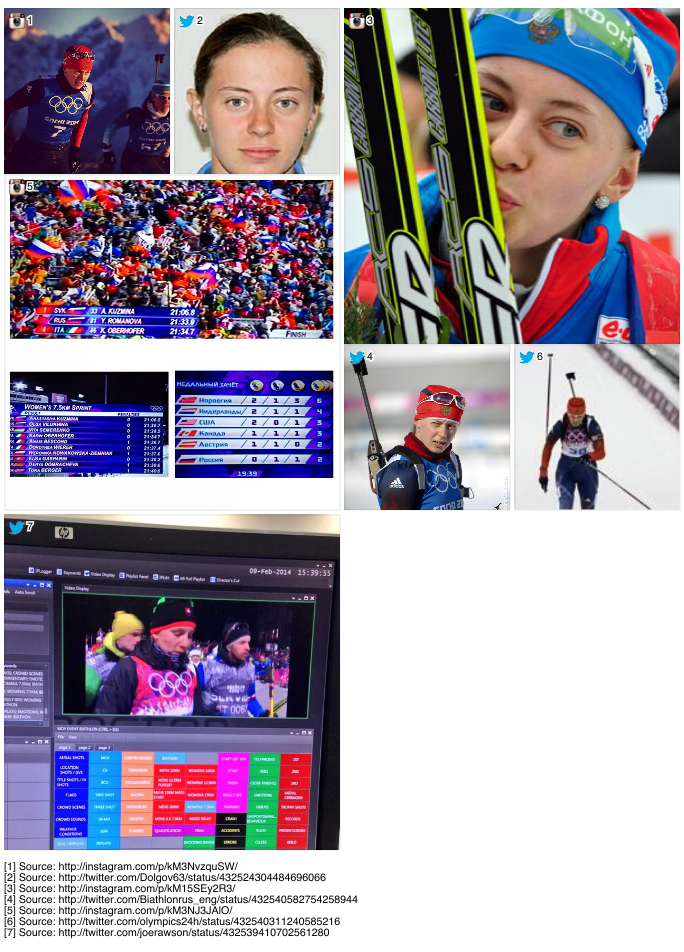
\includegraphics[height=2.75cm]{figures/olga_vilukhina/mediagallery_looseOrder_1391962084554.png}
    \caption{Feb 09, 17:08:04}
    \label{fig:1391962084554}
  \end{subfigure}%
  \begin{subfigure}[t]{0.25\textwidth}
    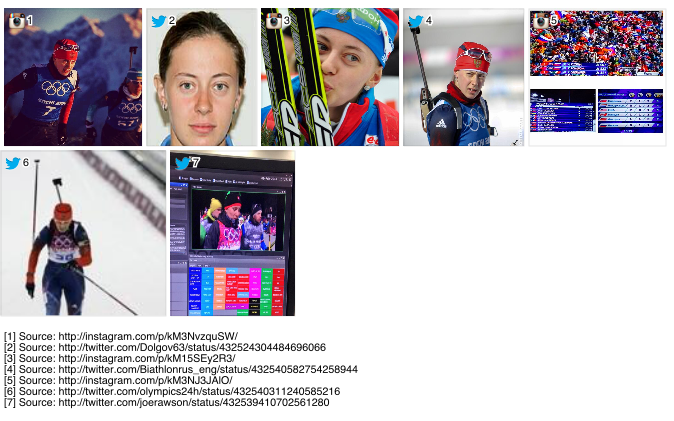
\includegraphics[height=2.75cm]{figures/olga_vilukhina/mediagallery_strictOrder_1391962084361.png}
    \caption{Feb 09, 17:08:04}
    \label{fig:1391962084361}
  \end{subfigure}  
  \caption{Media galleries for Olga Vilukhina,
    Women's Biathlon Sprint silver medal winner
    (times in CET, left: \emph{Loose Order, Varying Size},
    right: \emph{Strict Order, Equal Size})
    \url{https://twitter.com/WikiLiveMon/status/432540589700046848}}
  \label{fig:olga-vilukhina}
\end{figure}

\begin{figure}[t!]
  \centering
  % row 1
  \begin{subfigure}[t]{0.25\textwidth}
    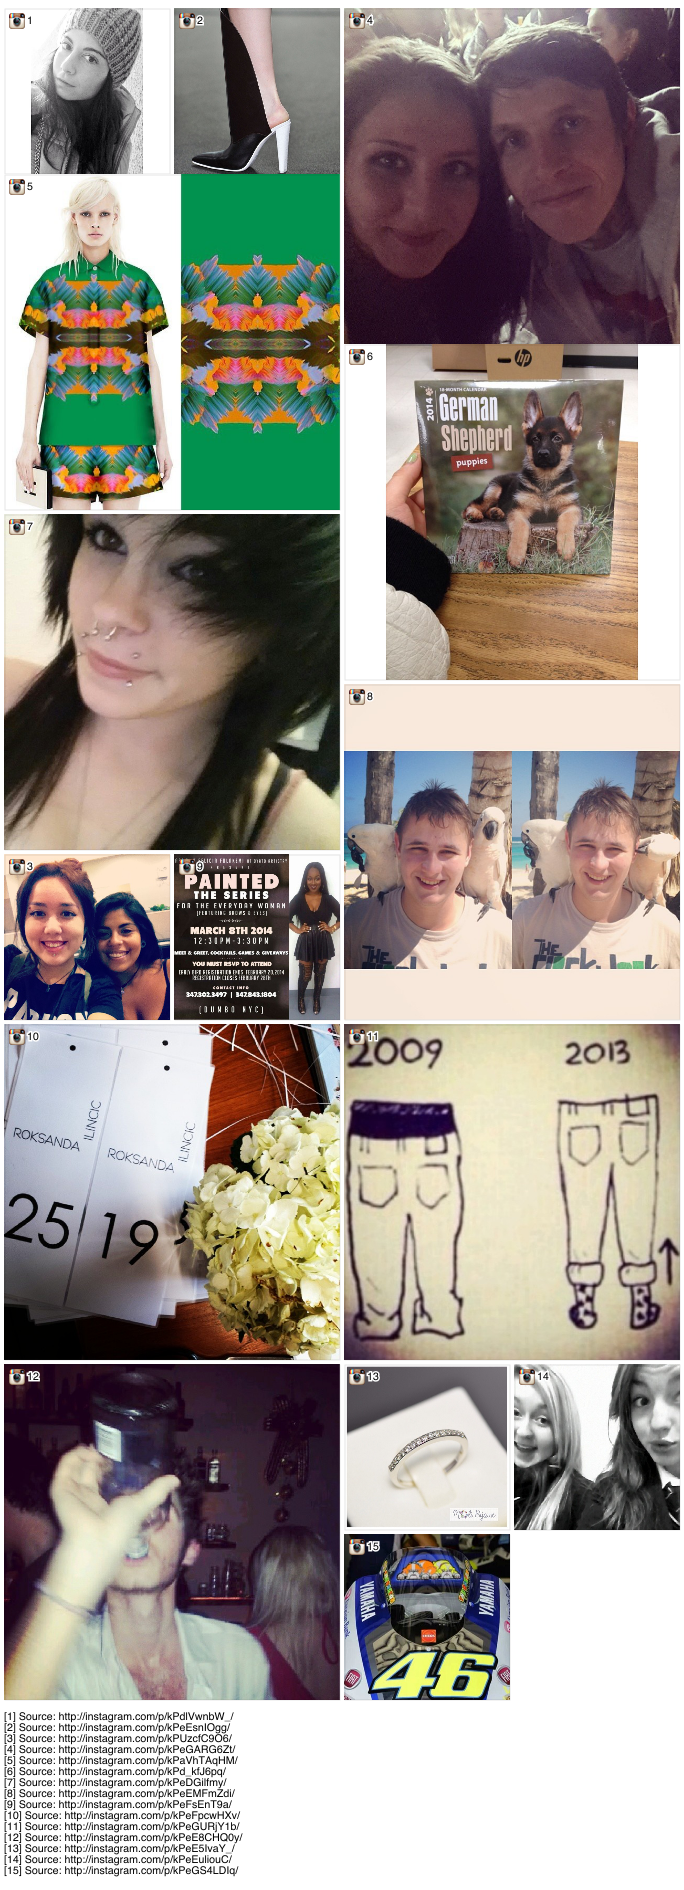
\includegraphics[height=5.25cm]{figures/medal_table/mediagallery_looseOrder_1392048536608.png}
    \caption{Feb 10, 17:08:56}
    \label{fig:1392048536608}
  \end{subfigure}%
  \begin{subfigure}[t]{0.25\textwidth}
    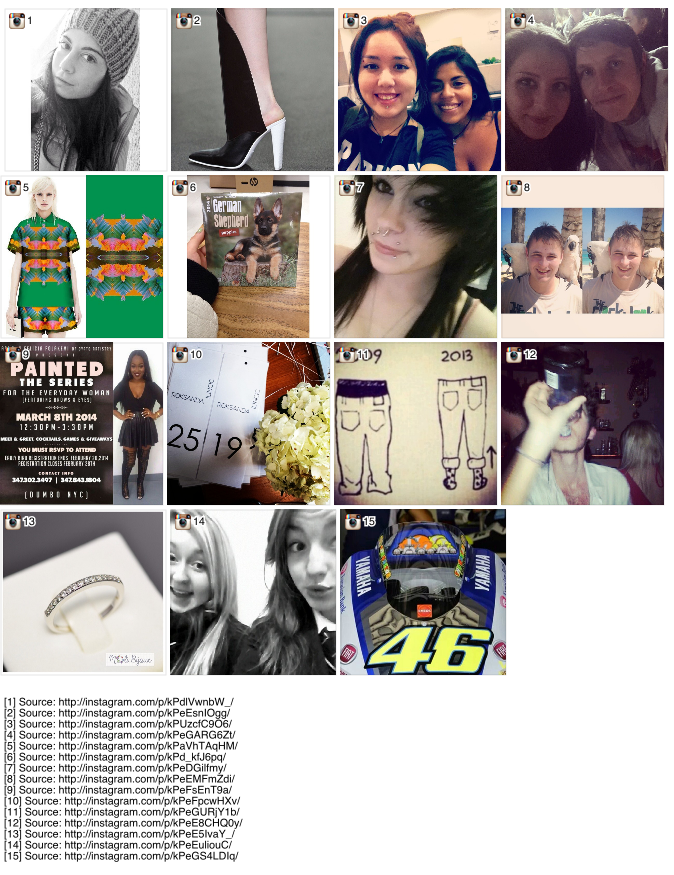
\includegraphics[height=5.25cm]{figures/medal_table/mediagallery_strictOrder_1392048536209.png}
    \caption{Feb 10, 17:08:56}
    \label{fig:1392048536209}
  \end{subfigure}
  \caption{Completely irrelevant media gallery for
    \emph{2014 Winter Olympics medal table}
    (times in CET, left: \emph{Loose Order, Varying Size},
    right: \emph{Strict Order, Equal Size})    
    \url{https://twitter.com/WikiLiveMon/status/432909036313673728}}
  \label{fig:medal-table}
\end{figure}

\section{Related Work}
\label{sec:related-work}
\fontencoding{T1}\selectfont

We focus on related work that follows a~\emph{holistic approach}
for storytelling with social media
rather than looking at individual bits and pieces
like event detection, media deduplication and clustering, \emph{etc.}
Related work can be grouped in several fields.

\paragraph{Storytelling with Social Media Around the Olympics}

The Twitter data journalism team have created a~visualization
of the most-shared Olympics photos on Twitter%
~\cite{schweitzer2014twitter} that can be
filtered by day and country.
It is unclear to what extent the system is based
on automated hashtag analysis and manual content curation.
More visualizations like an interactive map
and an athlete follower graph
are listed in a~post on the Twitter blog~\cite{rogers2014twitter}.

\paragraph{Event Archiving and Summarization}

Event archiving services such as Eventifier%
\footnote{Eventifier: \url{http://eventifier.co/}} 
do a~great job at storing all the social media content around
entire events, however, do not currently rank the information.
Closest to our approach is Seen%
\footnote{Seen: \url{http://seen.co/}}
an engine that aggregates, organizes, and ranks media
and collects information on topics trending in social media.
Seen does not support tracking of media gallery evolution.
Finally there is MediaFinder~\cite{troncy2013mediafinder},%
\footnote{MediaFinder: \url{http://mediafinder.eurecom.fr/}}
that uses a~fork of the media item collector
used in \emph{Social Media Illustrator}
MediaFinder specializes on clustering media items
based on named entities.

\paragraph{Manual Social Multimedia Curation}

Examples of manual social media curation tools are FlypSite,%
\footnote{FlypSite: \url{http://www.flyp.tv/}}
a~tool that facilitates the creation of embeddable
second screen applications or TV social media widgets,
Storify~\cite{fincham2011storify,atasoy2011storify},%
\footnote{Storify: \url{http://storify.com/}}
a~social network service that lets users create stories
or timelines using social media, and Storyful,%
\footnote{Storyful: \url{http://storyful.com/}}
a~news agency focused on verifying and distributing
user-generated content from social networks related to news events.

\paragraph{Identification and Aesthetic Presentation}

Automated and semi-automated approaches for content identification exist,
for example, \cite{liu2011events} and \cite{liu2011socialmedia}
by Liu \emph{et~al.}\ who combine semantic inference
and visual analysis to automatically find media items
that illustrate events.
Further, there are \cite{becker2010eventidentification}
and \cite{becker2012plannedevents} by Becker \emph{et~al.}\
who focus on identifying media items related to events
by learning similarity metrics and identifying search terms.
However, these event-related social multimedia data
identification approaches do not deal with the tasks of
ranking~\cite{liu2009learningtorank}, deduplicating~\cite{yang2009nearduplicate},
and representing the event-related content aesthetically%
~\cite{sandhaus2011photobook,obrador2012photoaesthetics}.
Obrador \emph{et~al.}\ present a~photo collection summarization system
that includes storytelling principles and face and image aesthetic ranking,
however, that is not interactive.

\section{Future Work and Conclusions}
\label{sec:future-work-and-conclusions}
\fontencoding{T1}\selectfont

\bibliographystyle{abbrv}
\bibliography{references}
\balancecolumns
\end{document}